\chapter{Analysis}
Overall, a total of two objectives is required for the project. In the first part, propose a novel machine learning to modeling different PUF(physical unclonable function)
behaviour, in particular arbiter PUF and XOR arbiter PUF. In the second part, consider reconfigurability like adding noise, one-time-PUF to resilient against the modeling attack
proposed in part one.

\section{Project Aims and Evaluation}
The aims for part one are that the machine learning for modeling should be related to ETA(estimated time arrival) problem or the one people haven't used for modeling
PUF. Moreover, reconfigurability needs to be considered when proposing the modeling attack while knowing the PUF can escape from it by changing CRPs behaviours in part 
two. Therefore, machine learning should ideally adapt to the changing behaviour of CRPs or the PUF. For example, unsupervised learning can be a good way since it can 
deal with unseen data. To evaluate the work, an overall accuracy of the modeling are expected to be around 90\% and take short time like the logistic regression in 
paper \cite{Reference6}. In addition, the modeling attack should apply to a range of arbiter PUF and compare the experiment result.

The aim for part two is to propose a reconfigurability framework for the modeling attack in part one. Two different reconfigurability will be implemented. First, add intentional
noise to PUF's response during the authentication phase to disturb the modeling attack \cite{Reference8}. The basic idea is shown in Figure \ref{fig:figure10}, assuming the database has stored PUF's CRPs and provided a challenge c
to PUF in the authentication phase. The PUF return a response r', and add noise e with r'. Then e and r' compose helper data h and send back to the verifier, where $h = r'\oplus e$. The verifier can reproduce $r'\oplus e$  
with r and h if r and $r'\oplus e$ is similar. Last, the verifier send a arbitrary number x to user, both verifier and user create their own hashtag and compare to check if authenticate. In this case, because the attacker cannot accesses to r, they can only model based on c and $r'\oplus e$, the modeling
might not be accurate, tha only thing attacker can do is try to build model that with high prediction accuracy based on $r'\oplus e$. To evaluate the work of adding intentional noise, the modeling attack proposed in part one should have a reasonable accuracy drop(3-4\% according to \cite{Reference8}) and the authentication will still work 
though noise is added.

\begin{figure}[htp]
    \centering
    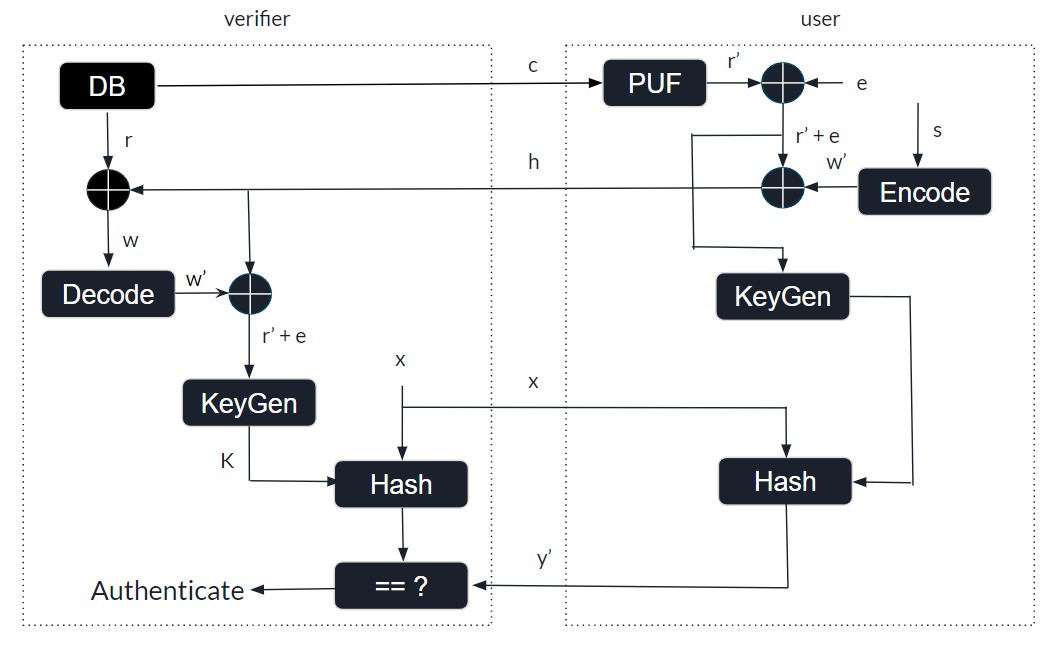
\includegraphics[width=18cm]{figures/figure10.jpg}
    \caption{Add noise to PUF's response during authentication phase \cite{Reference8}}
    \label{fig:figure10}
    \end{figure}

Second, implement protection which refers to OPUF to change the behaviour of CRPs and prevent modeling attacks. With control of parameters like refreshed-pause timing and allocating memory block, 
the project will examine the result of the protection. For example, evaluate the accuracy and time consumed when applying the modeling attack in part one.






